The ttbb 4FS Shape nuisance parameter has large pull in the S+B fit for all the mass points. Therefore S+B fit test is done with decorrelated ttbb 4FS across regions at 900 GeV mass point where the ttbb 4FS Shape mostly pulls to which regions are mostly fixed by this nuisance parameter.

Figure \ref{fig:ttbb_4FS_NP} shows the nuisance parameter pull of the fit test. Regions ljets\_ge10j3bL and os2l\_6jge4b are found to be mostly fixed by the ttbb 4FS Shape. Figure \ref{fig:ttbb_4FS_red_blue_pre_fit} show the red-blue plotsm of the ttbb 4FS Shape in the 2 regions and the pre-fit plots of the regions.

\begin{figure}
    \centering
    \begin{subfigure}[t]{0.49\textwidth}
      
\includegraphics[width=1 \textwidth]{figures/ttbb_4FS_decorrelation/NuisPar_ttbar.pdf}
    \end{subfigure}
    \caption{\label{fig:ttbb_4FS_NP}Nuisance Parameter pulls of S+B fit at 900 GeV mass point with decorrelated ttb 4FS uncertainty}
\end{figure}

\begin{figure}
    \centering
    \begin{subfigure}[t]{0.49\textwidth}
      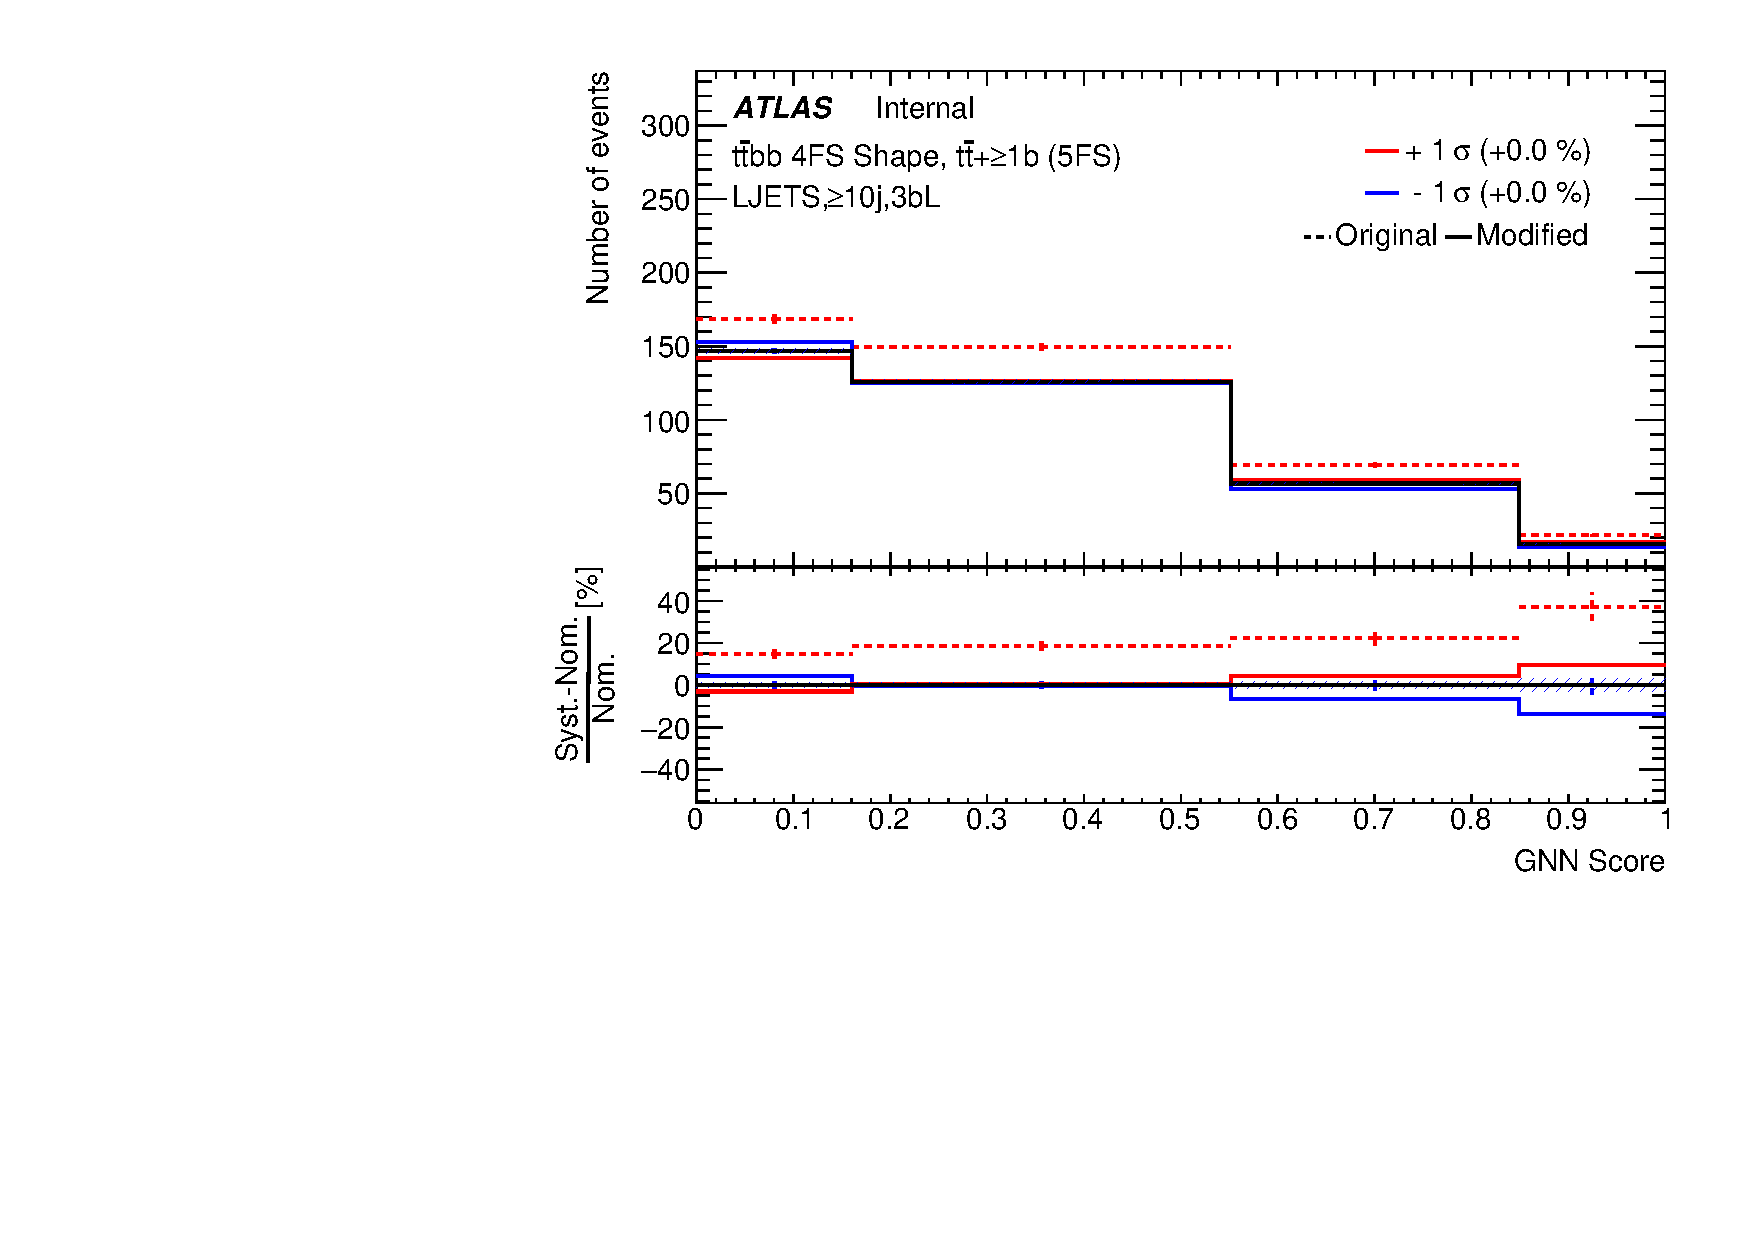
\includegraphics[width=1 \textwidth]{figures/ttbb_4FS_decorrelation/Red_blue_ljets_ge10j3bL.pdf}
      \caption{Red-blue plot on ljets\_ge10j3bL}
    \end{subfigure}
    \begin{subfigure}[t]{0.315\textwidth}
      
\includegraphics[width=1 \textwidth]{figures/ttbb_4FS_decorrelation/ljets_ge10j3bL.pdf}
      \caption{Pre-fit plot on ljets\_ge10j3bL}
    \end{subfigure}
    \\
    \begin{subfigure}[t]{0.49\textwidth}
        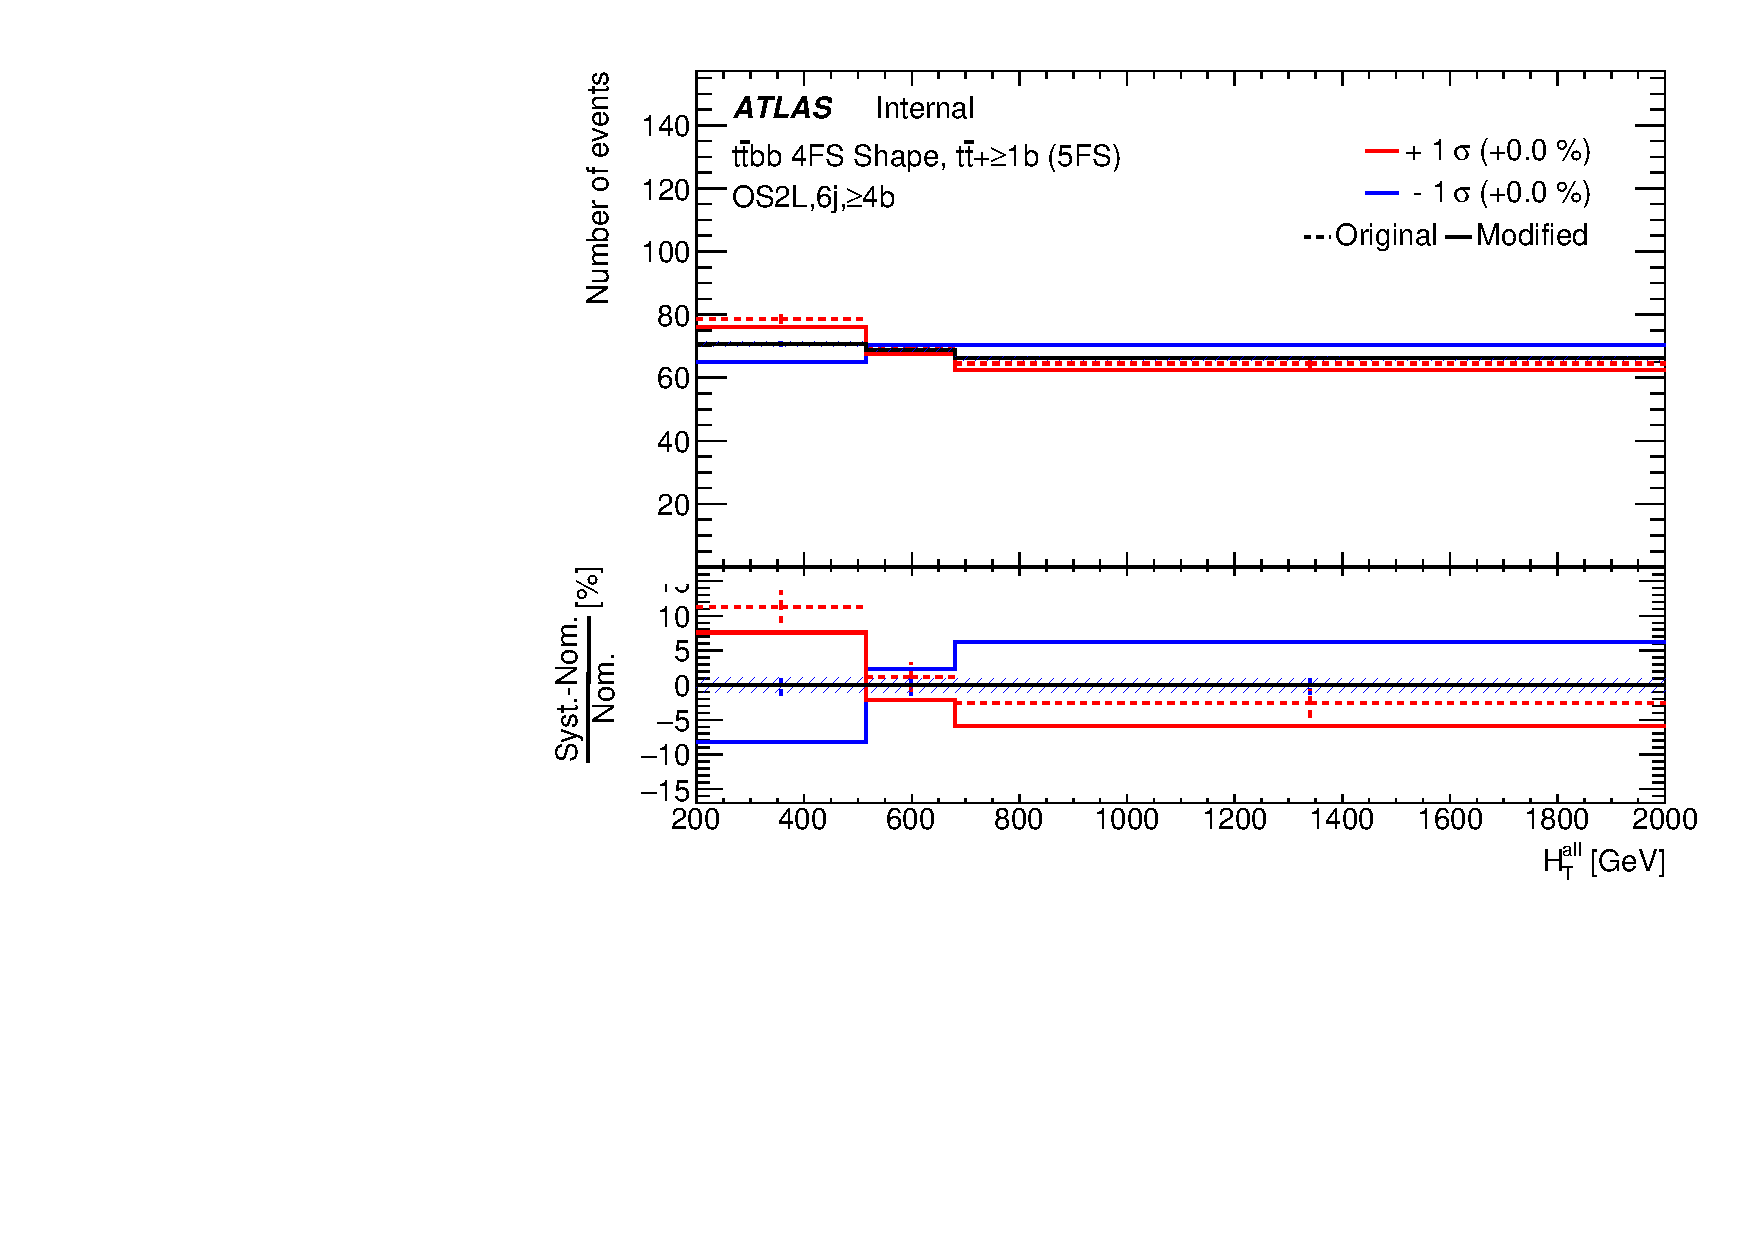
\includegraphics[width=1 \textwidth]{figures/ttbb_4FS_decorrelation/Red_blue_os2l_6jge4b.pdf}
        \caption{Red-blue plot on os2l\_6jge4b}
      \end{subfigure}
      \begin{subfigure}[t]{0.315\textwidth}
        
\includegraphics[width=1 \textwidth]{figures/ttbb_4FS_decorrelation/os2l_6jge4b.pdf}
        \caption{Pre-fit plot on os2l\_6jge4b}
      \end{subfigure}
    \caption{\label{fig:ttbb_4FS_red_blue_pre_fit}Red-blue plots of the ttbb 4FS Shape and pre-fit plots on ljets\_ge10j3bL and os2l\_6jge4b}
\end{figure}

The same test has been done at 400GeV mass point to check the constraint on the ttbb 4FS Shape nuisance parameter.
Figure \ref{fig:ttbb_4FS_NP_400} shows the nuisance parameter pull of the fit test. The strongest constraint comes from region ljets\_ge10j4b.

\begin{figure}
    \centering
    \begin{subfigure}[t]{0.49\textwidth}
      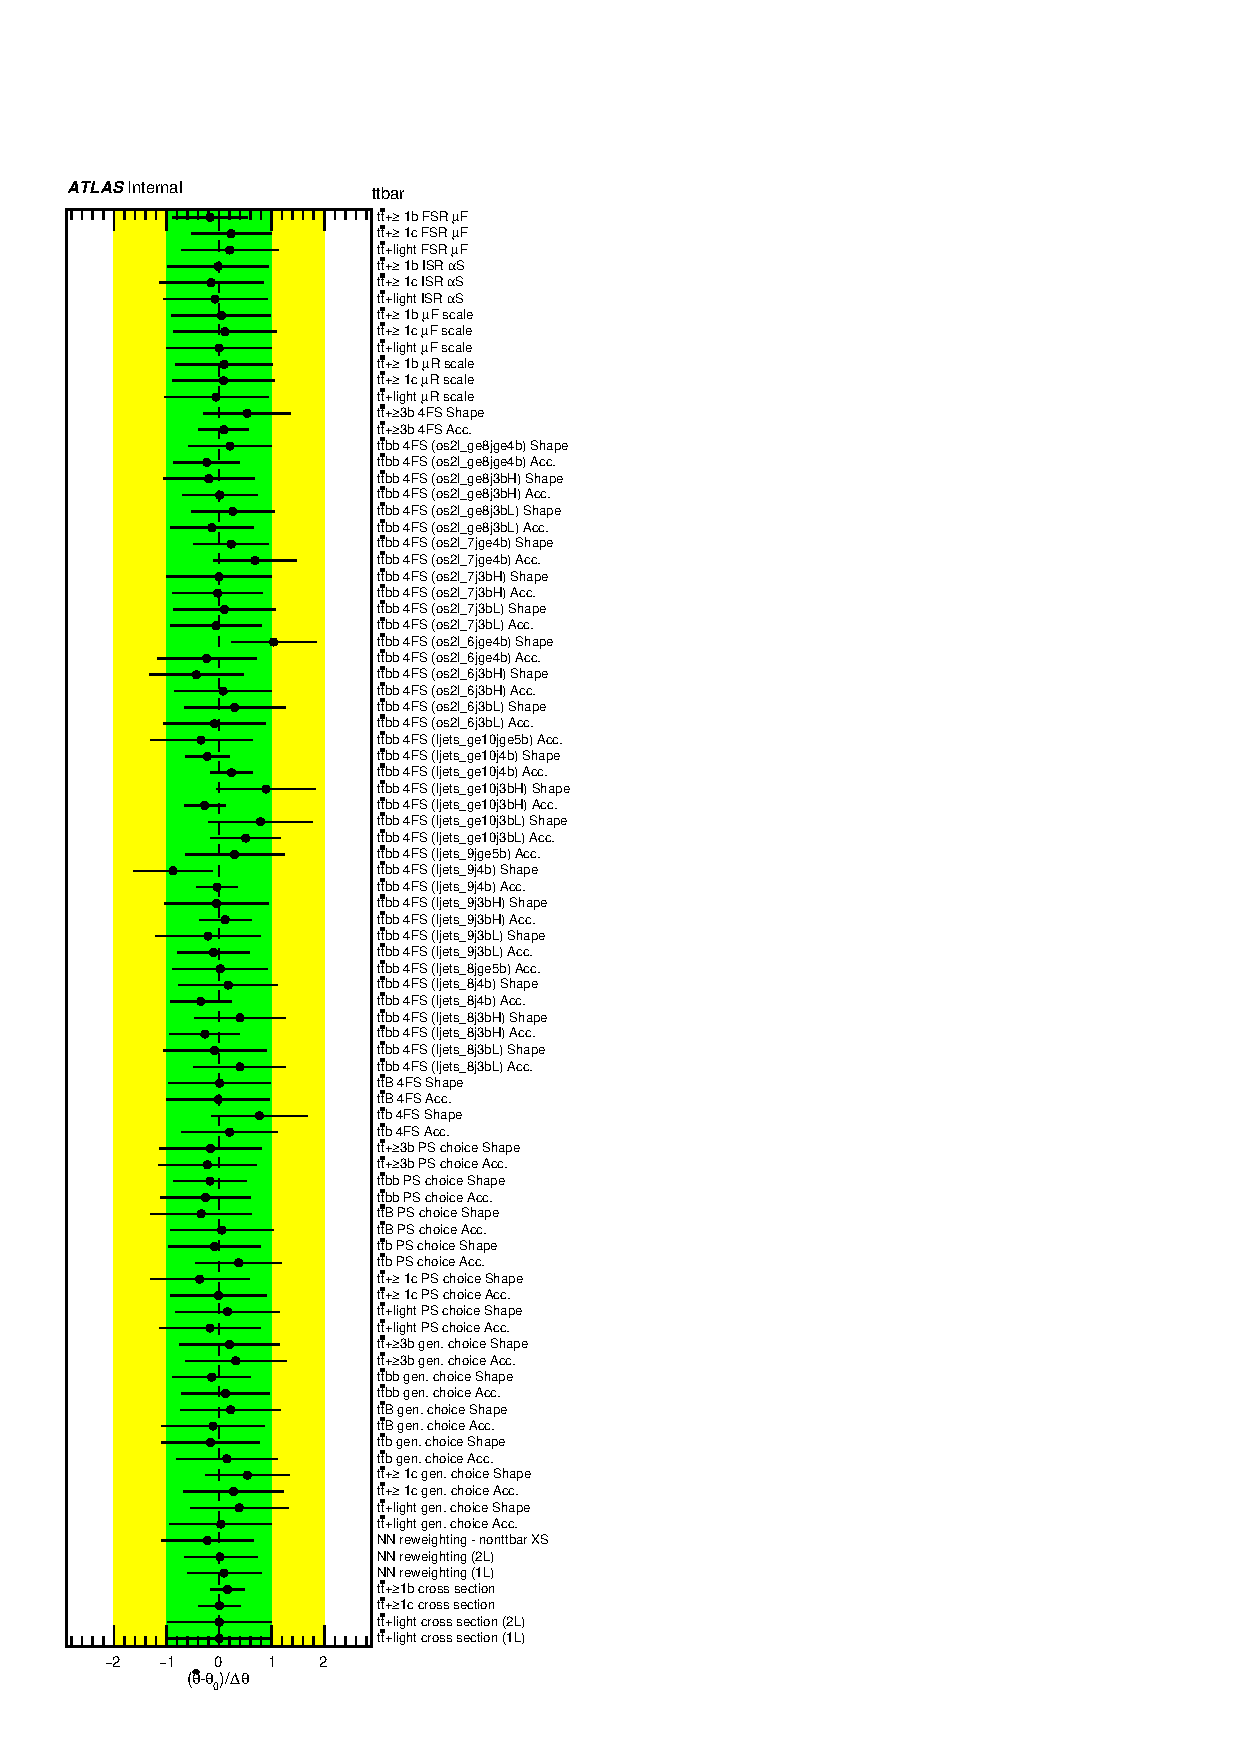
\includegraphics[width=1 \textwidth]{figures/ttbb_4FS_decorrelation/NuisPar_ttbar_400GeV.pdf}
    \end{subfigure}
    \caption{\label{fig:ttbb_4FS_NP_400}Nuisance Parameter pulls of S+B fit at 400 GeV mass point with decorrelated ttb 4FS uncertainty}
\end{figure}